
\documentclass[titlepage = firstcover]{scrartcl}
\usepackage[aux]{rerunfilecheck}
\usepackage{fontspec}
\usepackage[main=ngerman, english, french]{babel}

% mehr Pakete hier
\usepackage{expl3}
\usepackage{xparse}

%Mathematik------------------------------------------------------
\usepackage{amsmath}   % unverzichtbare Mathe-Befehle
\usepackage{amssymb}   % viele Mathe-Symbole
\usepackage{mathtools} % Erweiterungen für amsmath
\usepackage[
  math-style=ISO,    % \
  bold-style=ISO,    % |
  sans-style=italic, % | ISO-Standard folgen
  nabla=upright,     % |
  partial=upright,   % /
]{unicode-math}% "Does exactly what it says on the tin."
\usepackage[section, below]{placeins}

% Laden von OTF-Mathefonts
% Ermöglich Unicode Eingabe von Zeichen: α statt \alpha

\setmathfont{Latin Modern Math}
%\setmathfont{Tex Gyre Pagella Math} % alternativ zu Latin Modern Math
\setmathfont{XITS Math}[range={scr, bfscr}]
\setmathfont{XITS Math}[range={cal, bfcal}, StylisticSet=1]

\AtBeginDocument{ % wird bei \begin{document}
  % werden sonst wieder von unicode-math überschrieben
  \RenewDocumentCommand \Re {} {\operatorname{Re}}
  \RenewDocumentCommand \Im {} {\operatorname{Im}}
}
\usepackage{mleftright}
\setlength{\delimitershortfall}{-1sp}
\usepackage[version=4]{mhchem}

%Sprache----------------------------------------------------------
\usepackage{microtype}
\usepackage{xfrac}
\usepackage[autostyle]{csquotes}    % babel
\usepackage[unicode, pdfusetitle]{hyperref}
\usepackage{bookmark}
\usepackage[shortcuts]{extdash}
%Einstellungen hier, z.B. Fonts
\usepackage{booktabs} % Tabellen


\title{V500 - Der Photoeffekt}
\author{
  David Gutnikov\\
  \href{mailto:david.gutnikov@udo.edu}{david.gutnikov@udo.edu}\\
  Lasse Sternemann\\
  \href{mailto:lasse.sternemann@udo.edu}{lasse.sternemann@udo.edu}
}
\date{Bearbeitet am 29.05.2020}

\begin{document}
    \maketitle
    \newpage
    \tableofcontents
    \newpage


    \section{Theoretische Grundlagen}
        \subsection{Physikalische Beschreibung des Lichts}
        Die physikalische Beschreibung des Lichts erfolgt entweder über das Korpuskelmodell, das das Licht als Teilchen ansieht oder das Wellenmodell, das gemäß seines Namens das Licht als Welle 
        beschreibt. Während das eine Modell eine experimentelle Beobachtung gut beschreibt, kann es bei einer anderen experimentellen Beobachtung versagen. Daher werden beide Modelle als Grenzfälle
        der Quantenelektrodynamik eingeführt, sodass diese über Nutzung der Grenzfälle alle Phänomene beschreiben kann. Bei Wechselwirkungen von Licht mit Materie wird das korpuskulare Modell 
        angewandt und bei Beschreibung von der Ausbreitung des Lichts oder Interferenzphänomenen das Wellenmodell angewendet.
        
        \subsection{Der Photoeffekt}
        Beim Photoeffekt kommt es zu einer Wechselwirkung zwischen einfallendem monochromatischen Licht und einer Metalloberfläche. Dementsprechend ist für die Beschreibung das korpuskulare Modell 
        notwendig. Daher wird das Licht als Quant beschrieben, dessen Energie $E=h \cdot \nu$ proportional zur Frequenz des Lichts ist. Wenn nun ein Elektron, das durch eine Energie, die der 
        Austrittsarbeit $\text{A}_{\text{k}}$ entspricht, in einer Metalloberfläche gebunden ist, kann es durch einfallende Lichtquanten aus dem Metall gelöst werden, sofern die Photonenenergie größer 
        gleich der Austrittsarbeit ist.

        \begin{equation*}
            h \cdot \nu \geqslant \text{A}_{\text{k}}
        \end{equation*}

        \noindent
        Da $\lambda = c \cdot \nu$ gilt, hängt die Bedingung zur Auslösung eines Elektrons aus der Oberfäche also nur von der Frequenz $\nu$ bzw. Wellenlänge $\lambda$ des Lichts ab. Wenn die 
        Photonenenergie größer als die Austrittsarbeit ist, wird die restliche Energie als kinetische Energie an das Elektron übergeben und es ergibt sich folgende Energiegleichung. 
        Dabei wird die kinetische Energie des Elektrons über dessen Masse $m_{\text{e}}$ und Geschwindigkeit $v$ ausgedrückt.
        
        \begin{equation}
            h \cdot \nu = \text{A}_{\text{k}} + \text{E}_{\text{Kin}} = \text{A}_{\text{k}} + \frac{1}{2} m_{\text{e}}v^2
            \label{eqn:Energiegleichung}
        \end{equation}

        \noindent
        Jedoch ist die Energie der ausgelösten Elektronen nicht immer gleich, da sie von der Energie abhängt, die das Elektron vor dem Auslösen aus der Oberfläche bereits inne hat. Diese 
        Energieverteilung wird in der Fermi-Dirac-Statistik beschrieben und hat zur Folge, dass die Elektronen schon in der Oberfläche deutlich verschiedene Energien inne haben. Diese 
        Energieunterschiede haben zur Folge, dass bei der Messung des Photoeffekts über die Gegenfeldmethode, der gemessene Photostrom proportional zu Quadrat der Gegenfeldspannung ist. 

        \begin{equation*}
            I_{\text{Ph}} \propto U^2
        \end{equation*}

        \FloatBarrier

                \begin{figure}[h]
                  \centering
                  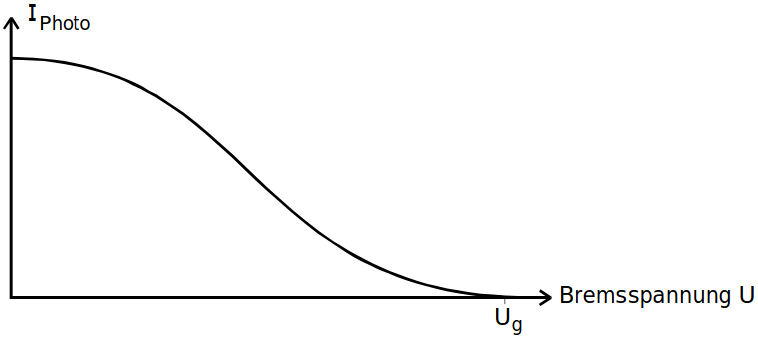
\includegraphics[width = 0.8\textwidth]{Bilder/IUTheorie.png}
                  \caption{In der Abbildung ist der schematische Aufbau zur Erzeugung von Spektrallicht und anschließender Aufteilung dieses in einzene monochromatische Strahlen zu sehen. Zudem ist ein Schwenkarm befestigt, der das Einstellen eines Schrims erlaubt, sodass immer nur ein monochromatischer Lichtstrahl durch die Schirmöffnung fällt. [1]}
                  \label{fig:IUTheorie}
                \end{figure}

        \FloatBarrier

        \noindent
        Über die beschrieben Theorie lässt sich folgern, dass es eine Grenzfrequenz geben muss, ab der das erste Mal Elektronen ausgelöst werden, dass die kinetische Energie der Elektronen
        proportional zur Frequenz $\nu$ des Lichts ist (\ref{eqn:Energiegleichung}) und dass die Anzahl der losgelösten Elektronen proportional zur Intensität des Lichts ist, da diese die Anzahl der 
        Photonen pro Zeit angibt und jedes Photon ein Elektron auslösen kann.


        \subsection{Elektronen im homogenen E-Feld}
        Freie Elektronen werden durch ein anliegendes, homogenes E-Feld beschleunigt und nehmen dabei eine elektrische Energie auf, die der kinetischen Energie des Elektrons nach der Beschleunigung
        im elektrischen Feld entspricht.

        \begin{equation}
            e \cdot U = \frac{1}{2} m_{\text{e}}v^2
            \label{eqn:Eel}
        \end{equation}

        \subsection{Gegenfeldmethode}
        Wenn die Photoelektronen aus einer Kathode ausgelöst werden, können sie auf eine aufgestellte Anode treffen und so einen Photostrom zwischen Kathode und Anode erzeugen. Dann wird zwischen
        Anode und Kathode eine regelbare Spannung gelegt, die die Elektronen entweder beschleunigt, "Beschleunigungsspannung", oder abbremst "Gegenfeldspannung". Mit steigender Gegenfeldspannung und 
        so steigendem E-Feld erreichen nur noch die energiereichsten Elektronen die Ringanode und bei noch weiterer Erhöhung über diese Grenzspannung $U_{\text{G}}$ wird garkein Strom mehr gemessen. 
        Durch Messung der Grenzspannung kann also bei Wissens der anderen Größen aus Gleichung \ref{eqn:Energiegleichung} und Einsetzens von Gleichung \ref{eqn:Eel} die Austrittsarbeit oder auch die 
        Energie oder Frequenz des Lichts über folgende Formel (\ref{eqn:Bestimmung}) bestimmt werden.

        \begin{equation}
          h \cdot \nu = \text{A}_{\text{k}} + \frac{1}{2} m_{\text{e}}v_{\text{max}}^2
          \label{eqn:Bestimmung}
        \end{equation}
        
        \noindent
        Ein mögliches Problem liegt auch in einer höheren Austrittsarbeit $A_A$ der Anode. Wenn diese mit der Kathode verbunden wird, passen sich die Fermi Niveaus an und trotz genügender Energie zum 
        Austreten aus der Phtokathode entsteht kein Photostrom, da die Photoelektronen ein "natürliches" Gegenfeld durchdringen müssten. In diesem Fall muss eine beschleunigende Spannung angelegt 
        werden, damit überhaupt ein Photostrom gemessen wird und dann wird diese gesenkt bis der Photostrom wieder auf Null fällt. Dieses Problem mit passender Lösung durch eine Beschleunigungsspannung
        ist in Abbildung \ref{fig:bSpannung} zu sehen.  

        \FloatBarrier

                \begin{figure}[h]
                  \centering
                  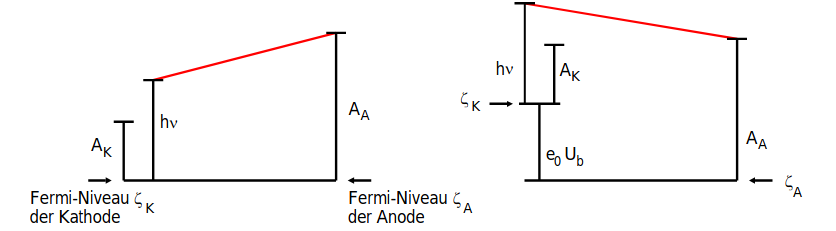
\includegraphics[width = 0.8\textwidth]{Bilder/bSpannug.png}
                  \caption{In der Abbildung ist die Energiedifferenz zwischen Photoelektronen an der Kathode und Anode zu sehen, die verdeutlicht warum trotz genügender Energie zum Photoeffekt kein Photostrom gemessen wird. Auf der rechten Seite ist die Erhöhung der Energie der Photoelektronen durch eine beschleunigende Spannung dargestellt. [1]}
                  \label{fig:bSpannung}
                \end{figure}

        \FloatBarrier

        \noindent



    \newpage
    \section{Aufbau und Durchführung}
        \subsection{Beleuchtung mit monochromatischen Licht}
            Um die Bestrahlung mit Licht einer einzelnen Wellenlänge zu ermöglichen, wird der in Abbildung \ref{fig:MonoLicht} zu sehende Aufbau verwendet. Die Spektrallampe emmitiert dabei Licht, dessen Wellenlängen 
            durch die Spektrallinien, des für die Lampe genutzen Materials begrenzt sind. Dieses Licht zunächst durch eine Abbildungslinse gebündelt wird und danach durch eine Spaltblende läuft, um 
            einen möglichst exakten Lichtstrahl zu erhalten. Dieser Lichtstrahl wird dann auf einen Prisma abgebildet, der das Licht in die einzelnen bereits erwähnten Spektrallinien zerlegt. Hinter 
            dem Prisma ist ein Schirm mit mittigem Eintritsspalt an einem Schwenkarm montiert, sodass die einzelnen Farben der Spektrallinien auf dem Schrim zu sehen sind und dieser so verstellt werden
            kann, dass immer nur das Licht einer Spektrallinie und somit einer Frequenz durchgelassen wird.
            
            \FloatBarrier

                \begin{figure}[h]
                  \centering
                  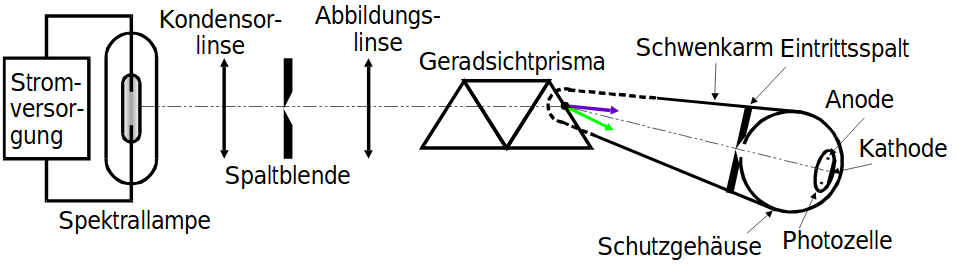
\includegraphics[width = 0.8\textwidth]{Bilder/Monolicht.png}
                  \caption{In der Abbildung ist der schematische Aufbau zur Erzeugung von Spektrallicht und anschließender Aufteilung dieses in einzene monochromatische Strahlen zu sehen. Zudem ist ein Schwenkarm befestigt, der das Einstellen eines Schirms erlaubt, sodass immer nur ein monochromatischer Lichtstrahl durch die Schirmöffnung fällt. [1]}
                  \label{fig:MonoLicht}
                \end{figure}

            \FloatBarrier

        \subsection{Photozelle}
            Der Photoeffekt wird letztendlich in einer Photozelle beobachtet. Diese ist in Abbildung \ref{fig:Photozelle} zu sehen und ist grundlegend ein evakuierter Glaskolben, zur Messung von Photoelektronen. In 
            diesem Glaskolben ist eine sogenannte Photokathode angebracht. Dabei handelt es sich um einen Schirm, der mit einer Metalllegierung bedampft worden ist, sodass bei Lichteinfall Elektronen 
            ausgelöst werden können. Wenige Zentimeter gegenüber der Photokathode befindet sich die zugehörige Ringanode.

            \FloatBarrier

                \begin{figure}[h]
                  \centering
                  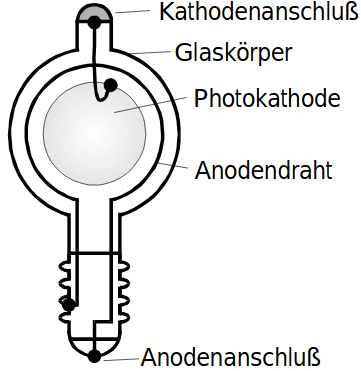
\includegraphics[width = 0.4\textwidth]{Bilder/Photozelle.png}
                  \caption{In der Abbildung ist der schematische Aufbau einer Photozelle zu sehen. [1]}
                  \label{fig:Photozelle}
                \end{figure}

            \FloatBarrier

            \noindent
            Zwischen Ringanode und Photokathode wird ein Picoamperemeter geschaltet, welches in der Lage ist den Strom zwischen Photokathode und Ringanode zu messen. Dieser Strom entsteht durch die
            ausgelösten Photoelektronen, die durch ihre kinetische Energie zur Ringanode fliegen und dort als Ladung aufgenommen werden. Zwischen Ringanode und Photokathode wird zudem ein elektrisches
            Gegenfeld angelegt, um die Gegenfeldmethode durchführen zu können.

            \FloatBarrier

                \begin{figure}[h]
                  \centering
                  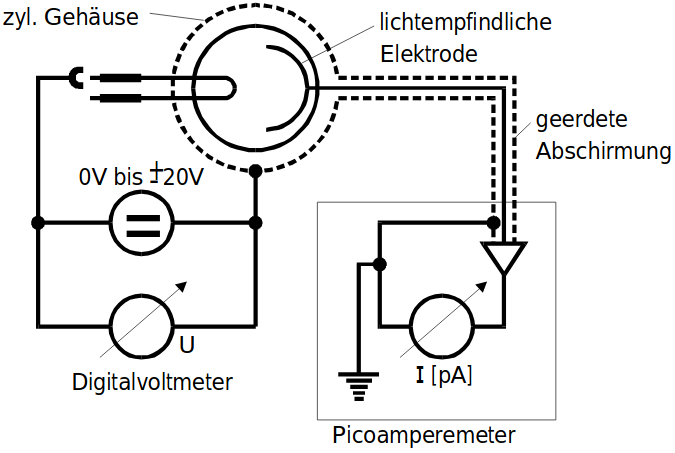
\includegraphics[width = 0.6\textwidth]{Bilder/Schaltung.png}
                  \caption{In der Abbildung ist der Schaltplan zur Erzeugung des Gegenfelds und Messung des Photostroms zwischen Photokathode und Ringanode zu sehen. [1]}
                  \label{fig:Schaltung}
                \end{figure}

            \FloatBarrier

        \newpage
        \subsection{Messungen des Photostroms}
            Mit Hilfe des beschriebenen Aufbaus wird zunächst für verschiedene Wellenlängen der Photostrom in Abhängigkeit von der angelegten Gegenspannung gemessen, um den in der Theorie
            beschriebenen Zusammenhang $I_{\text{Ph}} \propto U^2$ zu überprüfen. Dazu wird der Schwenkarm zuvor so bewegt, dass nur das Licht einer Wellenlänge auf die Photozelle trifft. 
            Daraufhin wird über die Steurungseinheit der Photozelle die Spannung in der Photozelle beginnend mit einer Beschleunigungsspannung heruntergeregelt bis keine Photostrom mehr auftritt. 
            Ist dies bei einer Spannung von 0 V nicht der Fall, wird auf eine Gegenspannung umgepolt und diese erhöht, bis der Photstrom auf Null fällt. Zunächst wird diese Messung im Abstand von 1 V
            Schritten durchgeführt, wenn ein linearer Zusammenhang zwischen Photostrom und SPannung aufzutreten scheint wird auf eine genauere Spannungsänderung angepasst. \newline
            
            \noindent
            Daraufhin wird unter konstanter Lichtintensität, sowie konstanter Lichtwellenlänge von $\lambda = 578 \, \text{nm}$ der Photostrom in Abhängigkeit von der angelgten Feldspannung gemessen.
            Ähnlich zur ersten SPannung wird nun wieder von einer beschleunigenden Spannung bis zu einer Gegenspannung variiert. Die Spannung startet mit einer Beschleunigenden Spannung von 20 V und 
            wird bis auf Null hinuntergeregelt und daraufhin auf eine Gegenspannung umgepolt und die Spannung erhöht bis der Photostrom wieder auf Null fällt. Auch hier wird im linearen Bereich mit 
            einer geringeren Spannungsänderung pro Messchritt gemessen.



    \end{document}

        